\chapter{Approach}

\section{Quadrotor Platform}
Because the design and construction of a quadrotor is beyond the scope of  this project, we will use a commercially available vehicle called the Bitcraze Crazyflie \cite{bitcraze}. The Crazyflie, shown in Figure \ref{fig:quad} is a small, low cost, open-source quadrotor kit suitable for indoor flight. It measures 9 cm motor to motor and weighs 19 grams. A 170 mAh lithium-polymer battery powers the vehicle, providing 7 minutes of flight time. An onboard microcontroller is responsible for vehicle stabilization and control and reads sensor measurements from a three-axis accelerometer, three-axis gyroscope, three-axis magnetometer, and barometer.
\begin{figure}[!htb]
\centering \includegraphics[scale=.15]{../fig/crazyflie.jpg}
\caption{Bitcraze Crazyflie Quadrotor}
\label{fig:quad}
\end{figure}

Vehicle pitch, roll, yaw, and thrust inputs are set in one of two ways. First, a USB gamepad connected to a computer running the Crazyflie PC client provides a method for direct user control of the vehicle. Second, the PC client exposes a Python API, making it possible to programmatically send the vehicle control set-points. The vehicle receives control inputs and transmits telemetry data wirelessly over a 2.4 GHz radio connection to a USB radio dongle connected to the Crazyflie PC client running on a laptop computer.
\begin{figure}[htb!]
	\centering
	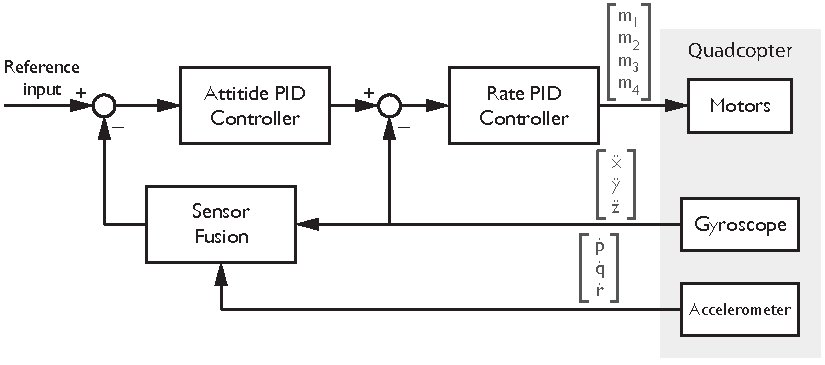
\includegraphics{../fig/crazyflie_control_system_block_diagram.pdf}
	\caption{Crazyflie control system block diagram}
\end{figure}

\section{Experiment Design}
blah
+persistence of excitation

\section{Data Collection}



\section{Data Analysis}
INCLUDE OVERVIEW OF IEM ALGORITHM IN BOX (MATH-BASED) IN THIS SECTION


\section{Verification}